\chapter{Estado de la cuestión}
\label{chap:Estado de la cuestion}
\Abstract{En este capítulo se desarrollará la situación sobre la que se desarrolla el proyecto. Se presentará la situación actual y se explicaran algunas de las herramientas y algoritmos usados en el proyecto.}

Como ya se ha indicado en la \autoref{chap:Introducción sec:Arquitectura}, este proyecto está claramente definido por dos elementos que deben de cooperar entre sí para poder cumplir el objetivo de identificar y recolectar las piezas. Se necesita de un buen sistema de reconocimiento de objetos a través de imágenes, así como de un brazo robótico para poder interactuar con el entorno. Por ello, se van a analizar cada uno de estos elementos por separado y después se desarrollará la interacción entre estos mismos. Primero se analizará la situación actual del procesado de imágenes, después se analizará los brazos robóticos y por último, se hablará de los sistemas \textit{Pick and Place}.

\section{Procesado de la imagen}
\label{chap:Estado de la cuestion sec:Procesado de la imagen}
Como ya se ha explicado en la introducción, los primeros sistemas de visión artificial surgieron en la década de los sesenta y desde entonces han avanzo notablemente hasta el nivel de convertirse en uno de los pilares fundamentales de la industria moderna. Actualmente los nuevos sistemas se han desviado drásticamente de los primeros intentos y emplean complejos sistemas neuronales y \textit{machine learning} para obtener mejores resultados y mejores respuestas. En este proyecto se va a perfeccionar el actual sistema basado en filtros de color y detección de borde y también se va a desarrollar una alternativa basada en redes neuronales.

\subsection{Filtros, detección de borde y detección de formas}
\label{chap:Estado de la cuestion sec:Procesado de la imagen subsec:Filtros, detección de borde y detección de formas}
La identificación de objetos no es un proceso directo, sino que está compuesto por varias etapas y dentro de estas existen multitud de herramientas. En esta sección se va a intentar segmentar este proceso y explicar de forma independiente cada proceso, así como las diferentes herramientas que se pueden usar.

\subsubsection*{Filtros}
Los filtros son diseñados con el objetivo de modificar la imagen para facilitar la extracción de características. Estos se pueden dividir en dos grandes categorías:

\begin{itemize}
\item \textbf{Filtros lineales:} Consisten en aplicar a cada píxel un filtro con sus píxeles vecinos. Dependiendo de los pesos que se den a los píxeles vecinos se pueden obtener diferentes efectos \cite{convolucion}. Se muestra la expresión matemática \ref{chap:Estado de la cuestion eq:CONV} que rige este proceso.

\begin{equation}\label{chap:Estado de la cuestion eq:CONV}
	g(i,j) =  \sum_{k,l}^{} f(i+k,j+l)*h(k,l)
\end{equation}
	
Se trata de un proceso por convolución en el que dependiendo de la matriz a usar y el peso de sus componentes se pueden obtener diferentes resultados \cite{convolucion}. Se puede ver su aplicación en la figura \ref{chap:Estado de la cuestion fig:CONV}.

\begin{figure}[ht]
	\centering
	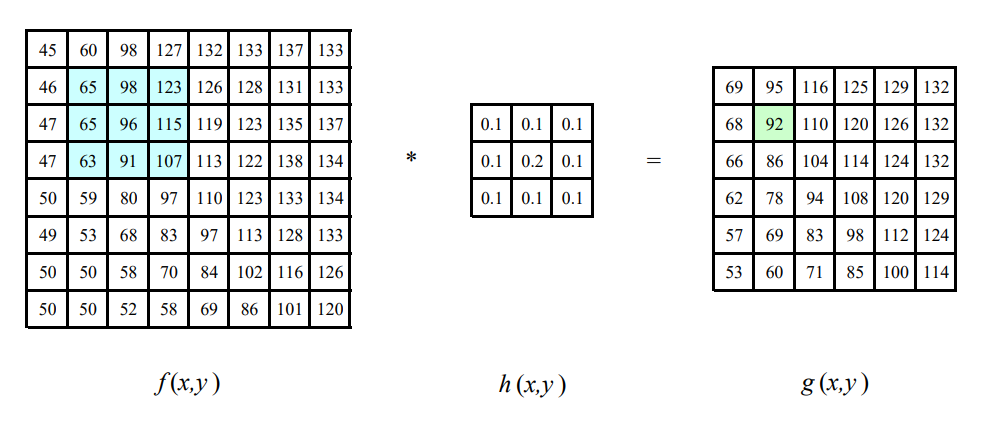
\includegraphics[width=0.8\textwidth]{EstadoDelArte/convolucion.png}
	\caption[Proceso de convolución en matrices]{Ejemplo de un proceso de convolución aplicado a una matriz (Fuente: Computer Vision: Algorithms and Applications, Richard Szeliski figure 3.10 \cite{szeliski})}
	\label{chap:Estado de la cuestion fig:CONV}
	\vspace{-5pt}
\end{figure}

Un claro ejemplo de este tipo de filtros es el suavizado. Permite suavizar la imagen y hacerla más homogénea al combinar cada pixel con sus vecinos. Este filtro permite reducir los valores atípicos reduciendo así el efecto del ruido. Pero también se puede dar el caso contrario en el que nos interese resaltar los pequeños detalles. Este filtro es conocido como \textit{Sharpening} y se basa en un filtro lineal de suavizado. A la imagen original se le resta las diferencias producidas por el suavizado y de esta forma se resaltan más los pequeños detalles de la imagen. Este proceso es conocido como \textit{unsharp masking} \cite{szeliski}.

\item \textbf{Filtros no lineales:} A pesar de que muchos de los filtros usados se pueden obtener de forma lineal, en muchas ocasiones se consigue un mejor rendimiento aplicando filtros no lineales. Tal y como su nombre indica, esta categoría engloba todos aquellos filtros que no se puedan expresar como una suma de diferentes argumentos. 

El beneficio de los filtros no lineales se puede ver al aplicar transformaciones que usen por ejemplo la mediana. El cálculo de la mediana puede suponer una alta carga computacional frente al resto de filtros. Por eso se han desarrollado alternativas para mejorar su cálculo. Tales como \textit{$\alpha$-trimmed mean} \cite{alfa}.

Un buen ejemplo de filtro no lineal que emplee la mediana es la transformación a escala de grises. Se suele usar la mediana ya que es más robusta ante variaciones atípicas. En el reconocimiento de objetos es muy recomendable usar la escala de grises ya que se consigue una mejor detección de borde \cite{greyscale} y reduce la carga computacional al trabajar con una sola matriz (\textit{Black}) en lugar de tres (RGB). Existen múltiples algoritmos para transformar a escala de grises, aunque uno de los más empleados y que mejores resultados da para el reconocimiento de borde es \textit{Lightness color-to-greyscale conversión algorithm} \cite{greyscale}. Sin embargo, gracias a los avances en redes neuronales y a la mejoras computacionales los sistemas actuales no se ven tan limitados y por ello son capaces de trabajar con imágenes de alta resolución y los tres canales RGB.
\end{itemize}


\subsubsection*{Detección de bordes}
Los bordes son el pilar fundamental de la visión artificial. Representan la separación entre diferentes objetos y definen sus formas. En una imagen, un borde se define como un salto de la intensidad de los pixeles.

En la práctica, estos cambios no son tan bruscos, sino que se producen gradualmente a lo largo de varios pixeles. Por ello no son tan fáciles de detectar y suelen aparecer bordes residuales producidos por ruido y errores en la imagen. En la detección de borde existen dos claras vertientes, aquellos métodos que se basan en el gradiente y los que emplean el laplaciano.

\begin{itemize}
\item \textbf{Operadores basados en gradientes:} El gradiente de una función es la colección de todas las derivadas parciales en forma de vector. La dirección del vector es la de máximo crecimiento y su módulo es el valor de la pendiente \cite{khan}. Al aplicar este concepto a imágenes, podemos obtener para cada píxel un vector que indique la dirección en la que aumenta la intensidad y su módulo. Analizando los gradientes obtenidos con la ayuda de máscaras, podemos encontrar los bordes ya que se producen por un cambio brusco de intensidad.

Existen varios algoritmos basados en el gradiente, aunque algunos de los más conocidos son el de Robert, Prewitt y el de Sobel. La diferencia entre estos son las máscaras a aplicar. Robert es un operador diferencial discreto con una matriz de 2x2, mientras que Prewitt y Sobel emplean dos matrices de 3x3. Se puede ver una comparativa de estos en la Figura \ref{chap:Estado de la cuestion fig:EDGE}.

El principal inconveniente de estos operadores es su forma de representar los bordes ya que están definidas por una franja de pixeles y además se ven bastante afectados por el ruido. Por ello existen algoritmos basados en la segunda derivada (laplaciano) para delimitar más la región de borde y obtener una mayor precisión.
\end{itemize}

\begin{figure}[ht]
	\centering
	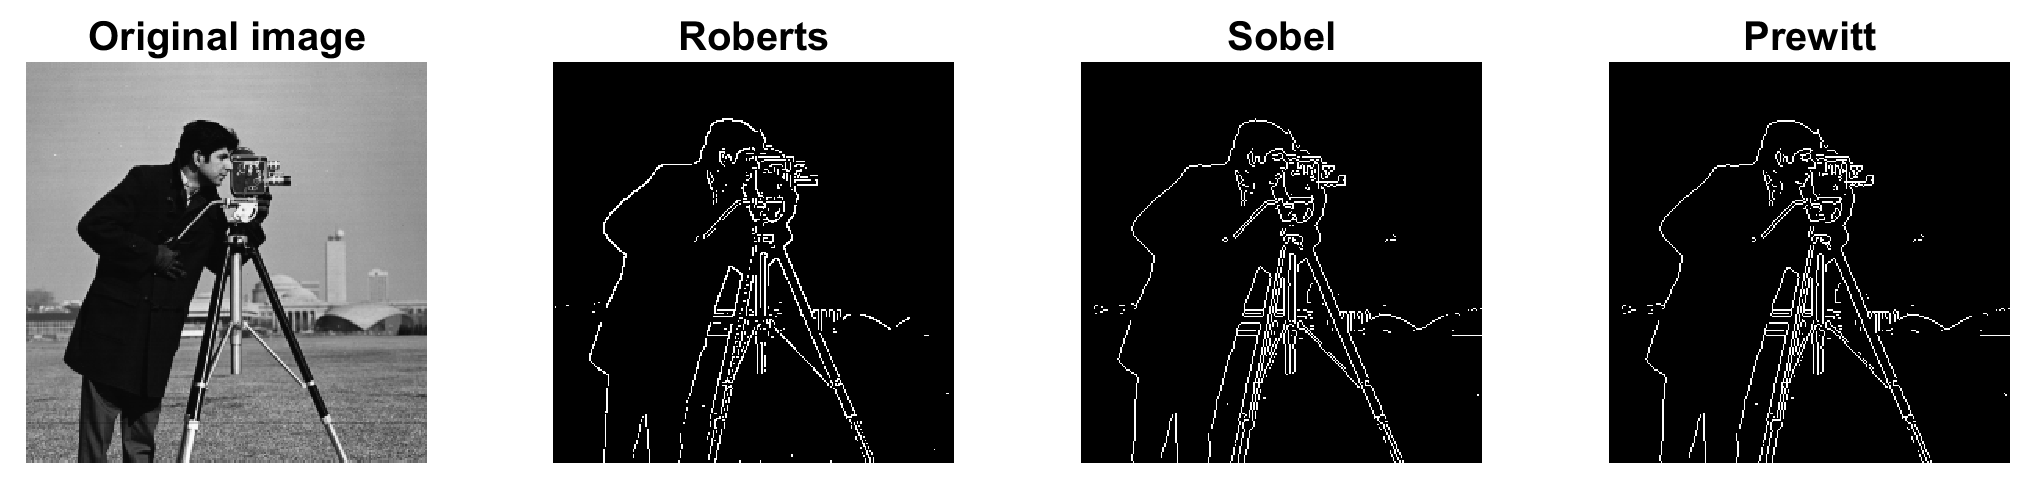
\includegraphics[width=0.9\textwidth]{EstadoDelArte/edge_detection_comparative.png}
	\caption[Comparativa de algoritmos de detección de borde]{Comparativa de algoritmos de detección de borde (Fuente: Ejemplo 		de MATLAB con imágenes de stock)}
	\label{chap:Estado de la cuestion fig:EDGE}
	\vspace{-5pt}
\end{figure}

\begin{itemize}
\item \textbf{Operadores basados en laplacianos:} Emplean la segunda derivada para obtener una mejor representación del borde y mayor robustez frente al ruido. Pero a cambio, requieren de una mayor carga computacional \cite{edgecomp}.

Existen múltiples algoritmos basados en el laplaciano, pero el más importante y usado es Canny. Esto es debido a su alto nivel de precisión y eficiencia. Asimismo, debido a su popularidad, han surgido múltiples variantes del algoritmo de Canny para perfeccionar la detección de borde.

El algoritmo de Canny se realiza en tres etapas. El primer paso es aplicar un filtro gaussiano para suavizar la imagen y evitar falsos bordes producidos por ruido en la imagen. A continuación, se calcula el gradiente de cada punto con su dirección y módulo. En este paso se intenta encontrar todos los bordes posibles de la imagen, pero con una diferencia respecto a los algoritmos anteriores, en este caso solo se queda con los máximos locales, convirtiendo así los bordes en líneas más nítidas y sin el efecto rampa. Por último, se hace un filtrado para eliminar los bordes innecesarios. Para ello se aplica un doble umbral sobre los gradientes y seguido por un rastreo de histéresis. Este elimina todos aquellos posibles puntos que no estén conectados a un borde. Se pueden observar los resultados en la Figura \ref{chap:Estado de la cuestion fig:EDGE2}.
\end{itemize}

\begin{figure}[ht]
	\centering
	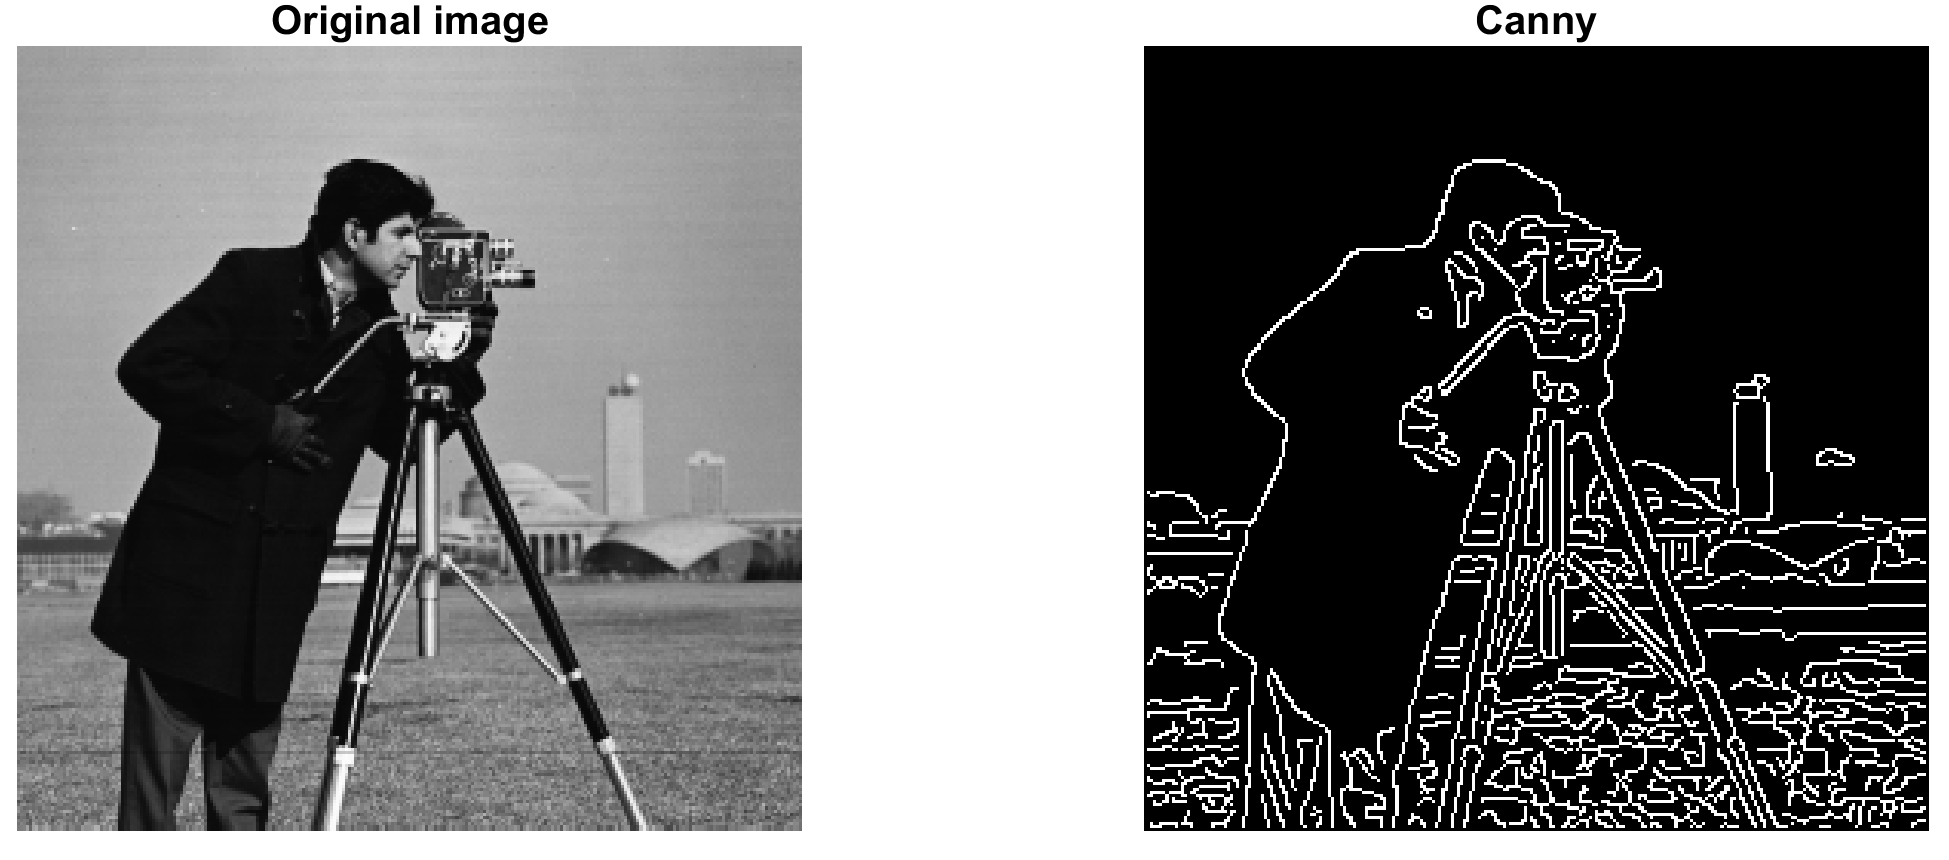
\includegraphics[width=0.8\textwidth]{EstadoDelArte/edge_detection_canny.png}
	\caption[Detección de borde por algoritmo de Canny]{Detección de borde por algoritmo de Canny (Fuente: Ejemplo de MATLAB con imágenes de stock)}
	\label{chap:Estado de la cuestion fig:EDGE2}
	\vspace{-5pt}
\end{figure}
	
\subsubsection*{Detección de formas}
Tras procesar la imagen y aplicar los algoritmos de detección de borde, se puede comenzar a analizar la escena. El objetivo de esta etapa es reconocer líneas y formas para poder detectar la posición y orientación del objeto. De nuevo, existen múltiples algoritmos para solventar el problema de localización y determinación a partir de imágenes. En este documento solo se van a analizar dos, la transformada de Hough y \acs{ransac} ya que en múltiples ocasiones han demostrado su robustez y son dos de los algoritmos más extendidos.

\begin{itemize}
\item \textbf{Transformada de Hough:} Este algoritmo fue diseñado en 1972 por Richard Duda y Peter Hart \cite{hough} y se ha postulado como una de las mejores alternativas para el reconocimiento de formas geométricas primitivas. Entendiéndose estas como una curva o superficie que pueda ser expresada matemáticamente con tres parámetros \cite{hough}. Por ejemplo, una línea, circulo, elipse, etc.

Para poder identificar curvas o superficies, el algoritmo analiza cada punto de la imagen y hace pasar por este todos los patrones posibles. Para cada punto se almacena $\rho$, que representa la distancia mínima entre la recta a analizar y el origen de coordenadas, esta viene dada por una perpendicular a la recta. Y $\theta$ que es el ángulo del vector director de esa recta \cite{hough2}. Esto se puede ver gráficamente en la Figura \ref{chap:Estado de la cuestion fig:Hough}.

La transformada de Hough ha demostrado numerosas veces su gran robustez para detectar patrones y líneas, pero a pesar de ello, presente un gran inconveniente que impide que sea usada tan extensamente. Requiere de una alta carga computacional ya que debe analizar cada punto de la imagen y almacenar todas las posibles rectas/formas. Por ello, se han desarrollado multitud de variantes del algoritmo original con el fin de o mejorarlo o reducir su carga. Algunas de las variantes más notables son:

\begin{itemize}
\item \textit{\ac{rht}}: Se basa en el algoritmo original, pero con la peculiaridad de que no necesita analizar todos los puntos de la imagen. El algoritmo intenta seleccionar de forma aleatoria puntos que puedan formar parte de una posible curva. De esta forma, se reduce bastante la carga computacional.
	
\item \textit{\ac{pht}}: Parte del esquema de acumulación del algoritmo original, pero difiere en el método de selección del siguiente punto a analizar. Selecciona un subconjunto a analizar en el que se ha incluido puntos previamente detectados como borde. De esta forma se reduce notablemente la carga computacional.
		
\item \textit{\ac{ppht}}: Partiendo de la imagen original, se seleccionan puntos de forma aleatoria y se analizan antes de pasar al siguiente. Para cada punto se observa si puede formar parte de una línea o no y se decide en base a los resultados obtenidos por los anteriores puntos. La principal ventaja de este algoritmo es la capacidad de poder ser interrumpido en cualquier momento y aun así dar buenos resultados. Pero es bastante susceptible a dar falsos positivos producidos por ruido en la imagen.
\end{itemize}

\end{itemize}

\begin{figure}[ht]
	\centering
	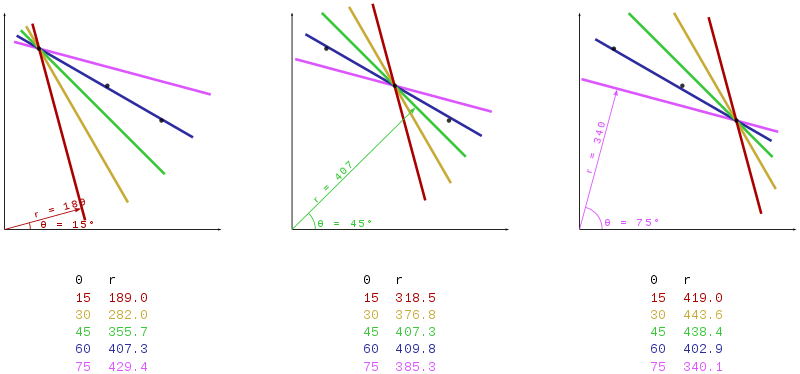
\includegraphics[width=0.7\textwidth]{EstadoDelArte/Hough_transform_diagram.png}
	\caption[Representación de la transforma de Hough]{Representación de la transforma de Hough (Fuente: \url{https://en.wikipedia.org/wiki/Hough_transform})}
	\label{chap:Estado de la cuestion fig:Hough}
	\vspace{-5pt}
\end{figure}

\begin{itemize}
\item \textbf{\textit{\acl{ransac}}:} También conocido como \acs{ransac}, se trata de un método matemático iterativo para encontrar los parámetros de un modelo matemático dentro de unos datos. Fue publicado por primera vez en 1981 por Fischler y Bolles y desde entonces se ha convertido en uno de los pilares de la visión artificial \cite{Fischler1981RandomSC}.

El método iterativo se puede separar en varias etapas que se repiten consecutivamente, tantas veces como se desee. Al aumentar el número de iteraciones, aumenta la probabilidad de detectar el objeto. Las etapas de cada iteración son:

\begin{itemize}
\item Selección de un subconjunto aleatorio sobre el que trabajar. Se conocen como \textit{inliers hipotéticos}.
\item  Basándose en el subconjunto, se monta un modelo sobre este.
\item Se comprueba la robustez del modelo contrastando contra el resto de los datos.
\item Si suficientes puntos se han clasificado como parte del modelo, este es válido.
\end{itemize}

En la siguiente iteración se partirá de este modelo y se intentará mejorar la detección de este.

Este algoritmo a pesar de ser muy preciso presenta una gran desventaja. Solo es capaz de contrastar la imagen frente a un modelo dado, por ello solo es capaz de detectar un tipo de objeto. Por ello se han desarrollado alternativas como \ac{r-ransac}.
\end{itemize}

\subsection{Redes neuronales convolucionales}
\label{chap:Estado de la cuestion sec:Procesado de la imagen subsec:Redes neuronales convolucionales}
La idea del aprendizaje automatizado/aprendizaje profundo/inteligencia artificial  no es novedosa, ya en 1955 IBM formó un grupo centrado en el reconocimiento de patrones supervisado por Nathaniel Rochester. Para ello, decidieron simular el funcionamiento de las neuronas con un ordenador IBM 704 \cite{Rochester}. Y aunque estos conceptos no suenan novedosos, es importante repasar los conceptos principales para poder entender las técnicas de aprendizaje automatizado \citep{alom2018history}.

En función del tipo de aprendizaje que se vaya a realizar, los tipos de inteligencias artificiales se pueden separar en 4 categorías:

\begin{itemize}
\item Aprendizaje supervisado: la información de la que se va a aprender ha sido preparada y etiquetada. Es un trabajo largo y tedioso, pero le permite a la inteligencia saber qué es lo que debe aprenderse.
\item Aprendizaje semi-supervisado: Tal y como su nombre indica, en este caso no toda la información ha sido preparada y etiquetada. 
\item Aprendizaje no supervisado: La información no ha sido preparada de ninguna forma y es el trabajo de la inteligencia el de entender la información y distinguir qué es lo que se desea aprender.
\item Aprendizaje por refuerzo: es un área del aprendizaje automático inspirada en la psicología conductista. La inteligencia debe de decidir que acciones tomar en un entorno y en función de sus decisiones recibirá una recompensa.
\end{itemize}

Qué tipo de aprendizaje usar depende del tipo de problema que se intente aprender. En este proyecto se va a emplear el aprendizaje supervisado. Para ello se emplearán imágenes previamente etiquetadas para que una red neuronal pueda aprender de ellas.

Desde la década de los cincuenta han surgido múltiples algoritmos para intentar simular el comportamiento de las neuronas y así poder alcanzar el objetivo de aprendizaje automatizado/profundo. Pero no fue hasta 1989 que surgió el concepto de Red Neuronal Convolucional impulsado por Yann LeCun. Yann desarrolló una de las primeras redes capaces del auto aprendizaje diseñada para reconocer la escritura a mano \cite{LeCun}. LeCun destacó por el uso de la convolución y fue uno de los primeros en obtener unos resultados positivos con este método.

En 2012 un grupo de investigadores dirigido por Alex Krizhevsky consiguieron obtener el menor error de clasificación visto hasta la fecha sobre las 1.2 millones de fotos de ImageNet con 1000 clases diferentes \cite{AlexNet}. Fue gracias a esta hazaña que empezó a crecer un gran interés por las redes neuronales convolucionales frente al resto de alternativas. Estas nuevas redes se basan en el principio de convolución, el cual ha sido explicado en la \autoref{chap:Estado de la cuestion sec:Procesado de la imagen subsec:Filtros, detección de borde y detección de formas}. La convolución se caracteriza por ser un proceso completamente lineal, esto es lo que ha permitido el desarrollo de estas redes y que puedan aprender tan fácilmente. En la actualidad este tipo de redes son las más comunes para el análisis de imágenes y su uso está ampliamente extendido.

Dentro del procesado de imágenes por aprendizaje profundo se distinguen dos categorías de redes en función de su objetivo:

\begin{itemize}
\item Clasificadores: son capaces de identificar un objeto en una imagen. Pueden ser entrenados para identificar una gran cantidad de objetos, pero tienen la desventaja de que solo pueden detectar un objeto por imagen. Además, solo indican su presencia, no su posición. Uno de los clasificadores más conocidos es AlexNet, la red neuronal diseñada por Alex Krizhevsky y mencionada anteriormente. Se muestra su estructura en \autoref{chap:Estado de la cuestion fig:AlexNet}.

\begin{figure}[ht]
	\centering
	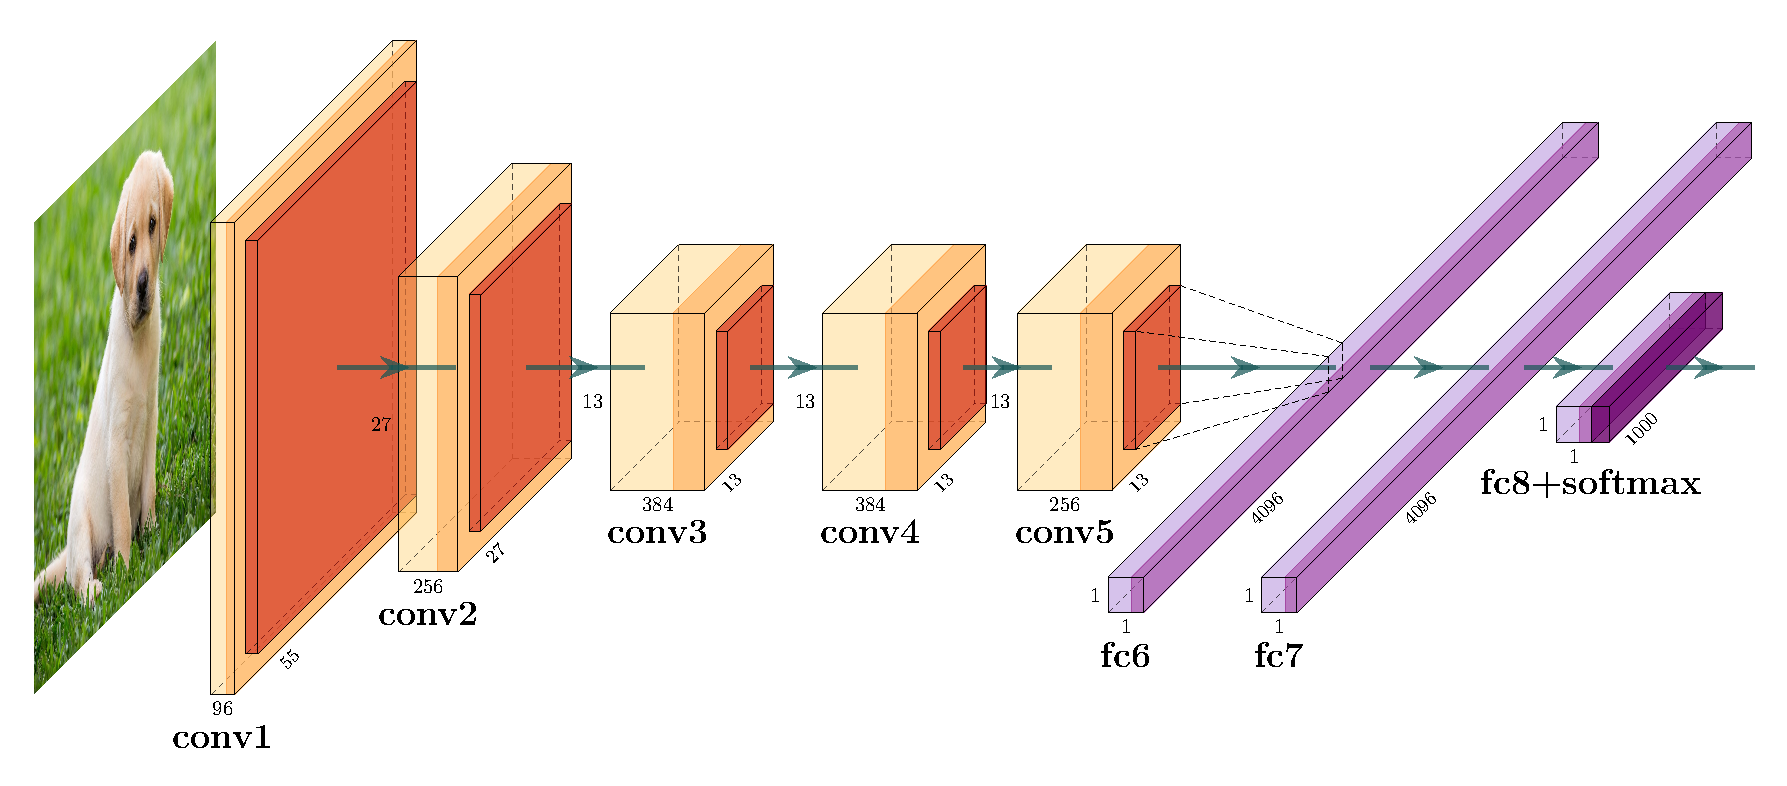
\includegraphics[width=0.9\textwidth]{EstadoDelArte/AlexNet.pdf}
	\caption[Estructura de AlexNet]{Representación de la estructura de AlexNet \cite{AlexNet}}
	\label{chap:Estado de la cuestion fig:AlexNet}
	\vspace{-5pt}
\end{figure}

En los últimos años los clasificadores han vivido una gran evolución y desarrollo y en parte esto es debido a la competición de ImageNet. Todos los años, investigadores de todo el mundo compiten por intentar obtener el mejor resultado al intentar clasificar millones de imágenes y mil clases. En la actualidad ImageNet cuenta con más de 14 millones de imágenes de alta resolución para ser clasificadas en mil clases. A continuación, se muestra en la \autoref{chap:Estado de la cuestion fig:ImageNet} el avance de las redes en este área analizando el error cometido por estas en ImageNet. Como referencia también se ha añadido el error medio cometido por los humanos. Se puede observar que algunas de las redes más modernas ya son capaces de superar al ojo humano en estas pruebas.

\begin{figure}[ht]
	\centering
	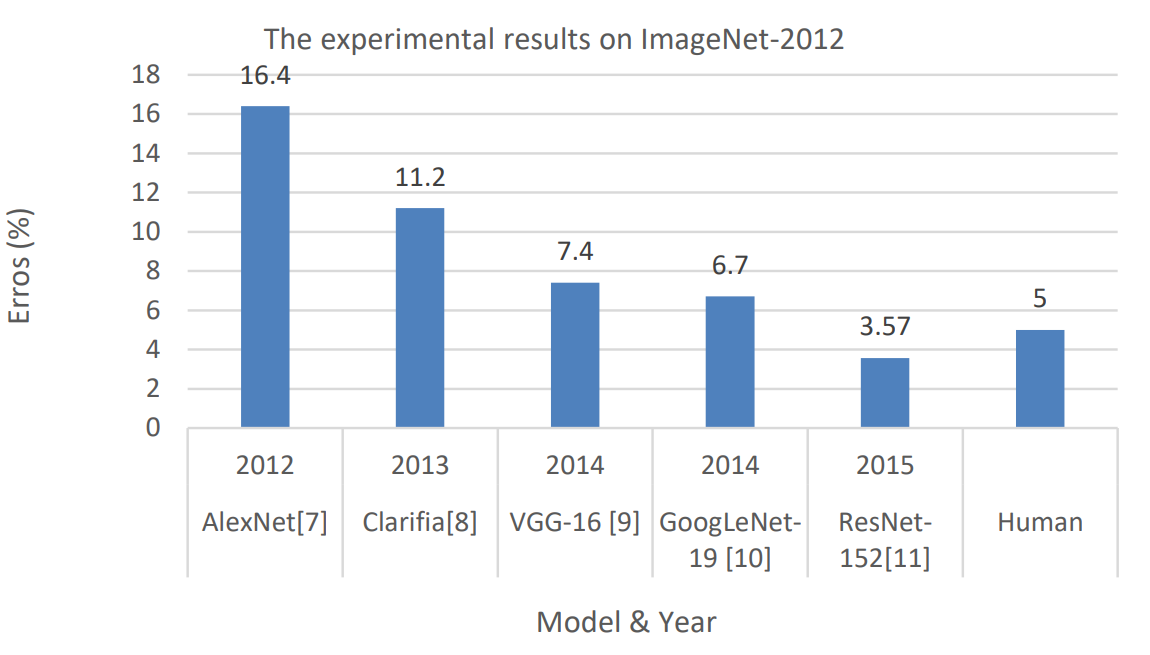
\includegraphics[width=0.7\textwidth]{EstadoDelArte/ImageNet.png}
	\caption[Errores cometidos en ImageNet en los últimos años]{Errores cometidos en ImageNet en los últimos años (Fuente: The History Began from AlexNet: A Comprehensive Survey on Deep Learning Approaches \cite{alom2018history}}
	\label{chap:Estado de la cuestion fig:ImageNet}
	\vspace{-5pt}
\end{figure}


\item Detectores de objetos: se basan en los principios de los clasificadores pero por medio de diferentes herramientas son también capaces de localizar el objeto en la imagen. Además, pueden identificar y detectar múltiples objetos en una misma imagen. En la actualidad existe una gran variedad de estructura y métodos para la detección de objetos, pero en este proyecto solo se van a analizar y emplear algunos de los más populares:

\begin{itemize}
\item \textit{\ac{r-cnn}}:Se basan en el principio de propuesta de regiones frente a sistemas empleados previamente conocidos como ventana flotante. Este sistema consiste en correr un clasificador barriendo todas las posibles secciones de una imagen y con diferentes tamaños. Como este proceso es muy costoso a nivel computacional y lento, \acs{r-cnn} propone usar un sistema que proponga un máximo de 2000 regiones a estudiar basándose en colores y formas fácilmente reconocibles. De esta forma se reduce bastante la carga, pero manteniendo un buen nivel de confianza y precisión.

\item \textit{\ac{faster-r-cnn}}: Al igual que \acs{r-cnn} se basan en el principio de propuesta de regiones pero difiere de este en el método para proponer dichas regiones de interés. En este método, la propia red neuronal se encarga de analizar la escena y decidir qué regiones debe considerar de interés. Esto resulta en una red bastante más rápida, aunque puede ser menos precisa que \acs{r-cnn}.

\item \textit{\ac{yolo}}: Es una de las técnicas más actuales y prósperas. Como su nombre indica, se caracteriza porque la imagen solo se pasa una vez por el clasificador y una capa convolucional se encarga de predecir la clase de objeto detectado y su posición. Este tipo de redes se caracterizan por ser extremadamente rápidas, aunque son incapaces de igualar la precisión de \acs{r-cnn}.
\end{itemize}
\end{itemize}


\section{Robótica industrial}
\label{chap:Estado de la cuestion sec:Robótica industrial}
El término robot se remonta hasta 1921 donde por primera vez se introdujo en la obra de teatro R.U.R (Rossum’s Universal Robots) obra del novelista y autor checo Karel Čapek. La palabra deriva de \textit{robota} que en checo significa fuerza del trabajo o servidumbre \cite{robotica}. En la actualidad es un término aceptado y conocido por toda la sociedad, empleado para designar a cualquier “máquina o ingenio electrónico programable que es capaz de manipular objetos y realizar diversas operaciones” (definición de robot según la RAE).

Actualmente los robots representan una gran parte de la fuerza de trabajo industrial. Se presentan en una gran variedad de configuraciones diferentes para cumplir diferentes objetivos, aunque una de las configuraciones más destacadas son los brazos robóticos. Tal y como su nombre indica, se asemejan a brazos de forma que tienen múltiples articulaciones sobre las que rotar para poder moverse en todas las direcciones y orientaciones posibles. 

Estos robots se pueden clasificar en función de diversas categorías:
\begin{itemize}
\item Por su función. Para ello se han desarrollado diferentes efectores que les permiten realizar tareas tan simples como \textit{Pick and Place} hasta tareas más exigentes como soldar.
		
\item Por su forma. Esta muchas veces se ve determinada por la función que debe desarrollar el brazo, así como el entorno en el que debe trabajar. Aunque a grandes rasgos se pueden distinguir dos tipos, fijos y móviles. Como sus nombres indican, esto depende de la capacidad del robot para moverse libremente.
		
\item Por el sistema de control. Los robots se pueden controlar por control manual, a distancia, mediante programación o con un sistema de aprendizaje por refuerzo.
		
\item Por el modelo de control de la planta. Una planta industrial dotada de numerosos robots tiene dos formas de ser controlada. Se puede tener un sistema de control independiente para cada robot, esto simplifica la creación de la planta, pero dificulta su manejo. O puede contar con un complejo sistema de interconexión entre las diferentes etapas de la planta. Un buen ejemplo de este tipo de sistemas de control es SCADA (Supervisory Control And Data Acquisition) \cite{SCADA}.
\end{itemize}

\begin{figure}[h]
	\centering
	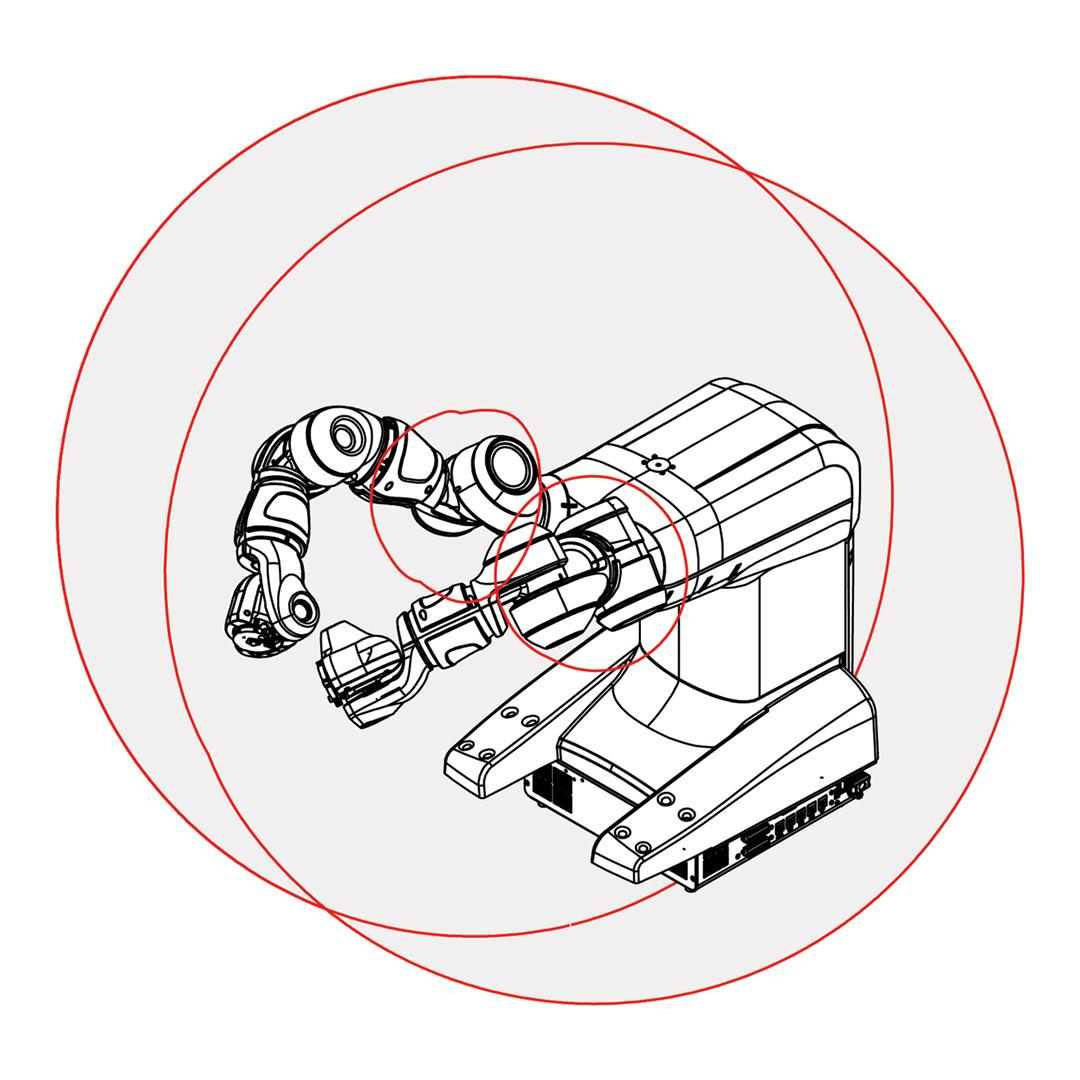
\includegraphics[width=0.6\textwidth]{EstadoDelArte/IRB1400.jpg}
	\caption[Brazo robótico IRB 1400 YuMi]{Brazo robótico IRB 1400 YuMi empleado en el proyecto con su rango de acción \cite{YuMi}}
	\label{chap:Estado de la cuestion fig:IRB1400}
	\vspace{-5pt}
\end{figure}

Como ya se ha explicado previamente, el objetivo de este proyecto es el desarrollo de un sistema capaz de localizar y capturar piezas para la preparación de un pedido. Este tipo de sistemas son conocidos como configuraciones \textit{Pick and Place} y son ampliamente usadas en la industria. Estos sistemas suelen estar constituidos por un brazo robot, una cámara y una unidad de procesamiento para analizar las imágenes. En función de los objetos que deben transportar, estos varían su forma de coger los objetos y sus cabezales.

Un buen ejemplo de la importancia de estos sistemas es \textit{Amazon Robotics Challenge}. Con el fin de mejorar los sistemas actuales y de buscar a los mejores en el sector, Amazon ha creado una competición entre alumnos universitarios para desarrollar el mejor sistema \textit{Pick and Place} \cite{amazon}. Estos sistemas se basan en redes neuronales muy avanzadas y desarrolladas tales como RefineNet \cite{amazon}.
